% ID: SEL-D0010-BA-E02
% ESTADO: validada. S011; tres pasadas del mismo autor, sin segundo revisor.
\textbf{a) Semiplanos y vértices.}\par\nopagebreak[4]
Despejamos $y$, invirtiendo la desigualdad cuando dividimos por un número negativo:
\[
y\geq\frac{5x+19}{4},\quad y\geq\frac{3x+13}{4},
\quad x\geq-7,\quad y\leq-x-2.
\]
La segunda y la cuarta implican $x\leq-3$. Para esos valores, la segunda cota inferior es mayor o igual que la primera, pues su diferencia es $-(x+3)/2\geq0$. La primera restricción no recorta más el recinto; se cumple con igualdad en $(-3,1)$.
En $x=-7$ las cotas activas dan $-2\leq y\leq5$; las dos fronteras oblicuas activas se cortan en $(-3,1)$. Por tanto, el recinto es el triángulo cerrado de vértices
\[
\boxed{(-7,-2),\quad(-3,1),\quad(-7,5).}
\]
No se añaden condiciones de no negatividad, que aquí eliminarían la región.
\begin{center}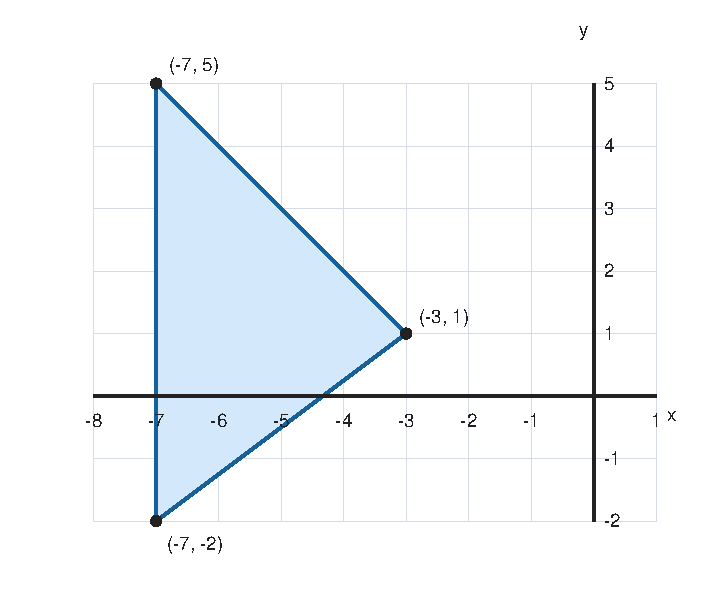
\includegraphics[width=0.56\linewidth]{recursos/figuras/s011-region.pdf}\end{center}

\textbf{b) Extremos de G.}\par\nopagebreak[4]
Una función lineal sobre un polígono compacto alcanza sus extremos en vértices. Evaluamos sin redondear:
\[
\begin{array}{c|rrr}
(x,y)&(-7,-2)&(-3,1)&(-7,5)\\\hline
G=-x/5+5y/2&-18/5&31/10&139/10
\end{array}
\]
\boxed{G_{\min}=-18/5\text{ en }(-7,-2)}, y \boxed{G_{\max}=139/10\text{ en }(-7,5)}. Ambos son únicos: los valores en los otros vértices son estrictamente intermedios.

\textbf{c) Valor propuesto.}\par\nopagebreak[4]
\[
\frac{47}{3}>\frac{139}{10},\qquad
\frac{47}{3}-\frac{139}{10}=\frac{53}{30}>0.
\]
\textbf{No puede alcanzarlo}: excede el máximo de $G$ en todo el recinto.
